\section{Durchführung}
\label{sec:Durchführung}

\subsection{Wheatstone Brücke}
\begin{figure}[H]
    \centering
        \centering
        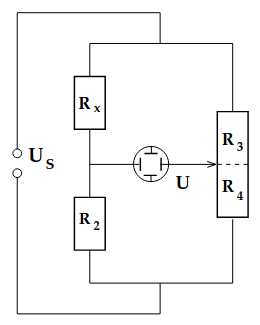
\includegraphics[width=0.35\textwidth]{Bilder/wheatstone.png}
        \caption{Wheatstone Brücke. \cite{anleitung}}
    \hfill
    \label{fig:f2}
\end{figure}
\noindent Bei der Wheatstone Brücke befinden sich nur Ohmsche Widerstände in 
dem Schaltkreis. Dabei liegen $R_3$ und $R_4$ am Potentiometer. Jenes ist
Spannungsteiler, an dem ein Schleifkontakt über den Widerstandtsdraht gelegt
wird, was es ermöglicht, den Widerstand kontinuierlich einzustellen. Um nun
den unbekannten Widerstand $R_x$ durch die Kompensationsmethode zu bestimmen, 
gilt
\begin{equation}
    \label{eqn:1}
    R_x = R_2 \frac{R_3}{R_4}.
\end{equation}
\noindent Als Einstellungen werden folgende Werte genommen:
\begin{align*}
    \label{eqn:werte1}
    \text{Potentiometer für } R_3 \text{ und } R_4 &= 1\,\unit{\kilo\ohm} \\
    \text{Frequenz } \nu &= 1\,\unit{\kilo\hertz} \\
    \text{Amplitude } U_{\text{S}} &= 1\,\unit{\volt} \\
    \text{Widerstand } R_2 &= 332;\, 664;\, 1000\,\unit{\ohm} \\
\end{align*}


\subsection{Kapazitätsmessbrücke}
\begin{figure}[H]
    \centering
        \centering
        \includegraphics[width=0.35\textwidth]{Bilder/kapazitätsmess.png}
        \caption{Kapazitätsmessbrücke. \cite{anleitung}}
    \hfill
    \label{fig:f3}
\end{figure}
\noindent Da in diesem Bereich des Experiments Kapazitäten bestimmt werden sollen, 
muss Wechselstrom verwendet weren. Es werden zwei Potentiometer verwendet, 
das erste wird wie gehabt als Spannungsteiler für $R_3$ und $R_4$ verwendet. Das 
zweite Poti wird als Spannungsteiler für die unbekannten Komponenten $C_x$ mit 
$R_x$ und der bekannten Kapazität $C_2$ genutzt.
\par\vspace{0.5em}
Die Brücke wird abgeglichen, indem alternierend die Poti so eingestellt werden, 
sodass die Spannung am Oszilloskop minimiert wird. Zuerst wird das eine Potentiometer 
so justiert, dass ein Minimum erreicht wird. Daraufhin wird das andere Poti so 
eingestellt, dass sich die Spannung weiterhin minimiert.
Dieses Verfahren wird so häufig wiederholt, bis die Brücke abgeglichen ist.
Für den Widerstand gilt weiterhin
\begin{equation}
    R_x = R_2 \frac{R_3}{R_4}.
\end{equation}
Für die zu bestimmende Kapazität dann:
\begin{equation}
    \label{eqn:2}
    C_x = C_2 \frac{R_4}{R_3}.
\end{equation}
\noindent Als Einstellungen werden folgende Werte genommen:
\begin{align*}
    \label{eqn:werte1}
    \text{Kapazität } C_2 &= 450;\, 597;\, 992\,\unit{\nano\farad} \\
    \text{Frequenz } \nu &= 1\,\unit{\kilo\hertz} \\
    \text{Amplitude } U_{\text{S}} &= 1\,\unit{\volt} \\
\end{align*}

\subsection{Induktivitätsmessbrücke}
\begin{figure}[H]
    \centering
        \centering
        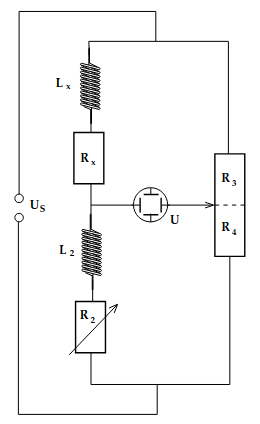
\includegraphics[width=0.35\textwidth]{Bilder/induktivitaetsmess.png}
        \caption{Induktivitätsmessbrücke. \cite{anleitung}}
    \hfill
    \label{fig:f4}
\end{figure}
\noindent Der Aufbau erfolgt analog zu dem der zuvor angesprochenen 
Kapazitätsmessbrücke. Es werden lediglich Kondensatoren mit Spulen ausgewechselt.
Folglich wird der Aufbau mit Wechselstrom betrieben. Für den unbekannten
Widerstand $R_x$ gilt erneut \autoref{eqn:1}. Eine Gleichung für die Induktivität
ergibt sich analog zu \autoref{eqn:2}:
\begin{equation}
    \label{eqn:3}
    L_x = L_2 \frac{R_4}{R_3}.
\end{equation}

\subsection{Wien-Robinson Messbrücke}
\begin{figure}[H]
    \centering
        \centering
        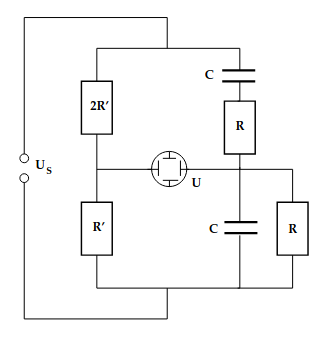
\includegraphics[width=0.35\textwidth]{Bilder/wien_robinson.png}
        \caption{Wien-Robinson Messbrücke. \cite{anleitung}}
    \hfill
    \label{fig:f5}
\end{figure}
Bei dieser Brücke, dessen Aufbau in \autoref{fig:f5} dargestellt ist, soll der 
Frequenzgang und der Klirrfaktor der Speisespannung ermittelt werden. Letzteres 
ist als Maß für die Qualität einer Spannungsquelle, insbesondere in Bezug auf 
die Reinheit der ausgegebenen Sinunsspannung, zu verstehen; er gibt an, wie 
stark die erzeugte Spannung von einer Sinuskurve abweicht. Gegensätzlich zu 
den vorherigen Versuchen wird diese Brücke nicht zur Messung von Komponenten 
genutzt, alle Komponenten verfügen über bekannte Werte. Die Brücke dient als 
elektronischer Filter für die Frequenz. Für das Verhältnis von Brückenspannung 
$U_{\text{Br}}$ zu der Speisespannung $U_{\text{S}}$ gilt:
\begin{equation}
    \left|\frac{U_{\text{Br}}}{U_{\text{S}}}\right|^2 = \frac{(\omega ^2 R^2 C^2 -1)^2}{9((1-R^2 C^2)^2+9 \: \omega ^2 R^2 C^2)}
\end{equation}
Bei Abgleichung der Brückenspannung (links) und der normierten Frequenz (rechts)
\begin{equation}
    \begin{aligned}
        \omega_0 &= \frac{1}{RC}, & \Omega &= \frac{\omega}{\omega_0}
    \end{aligned}
\end{equation}
reduziert sich das Verhältnis auf 
\begin{equation}
    \label{eqn:omega}
    \left|\frac{U_{\text{Br}}}{U_{\text{S}}}\right|^2 = \frac{9(\Omega ^2 -1)^2}{9(1-\Omega^2)^2+81 \: \omega ^2 \Omega^2}.
\end{equation}
Wie in der Theorie angemerkt, wird hier der Klirrfaktor relevant. Der Anteil der 
Oberwellen, welche detektierbar sind, werden durch eben diesen Faktor $k$ bestimmt. 
Dieser lautet
\begin{equation}
    \label{eqn:Klirrfaktor}
    k = \frac{\sqrt{\sum\limits_{i=2}^N U_i^2}}{U_1}
\end{equation}
mit der Amplitude der Grundwelle $U1$ und den Amplituden der i-ten Oberwellen 
$U_i$. Je näher der Klirrfaktor an dem Wert Null ist, desto weniger Oberwellen 
werde erzeugt.